The simple centroid readout is weak on raw held-out residuals, ranging from 25.0\% to 35.4\% across the sampled layers and positions (four-way chance: 25\%). Subtracting a matched no-secret state or the mean over secret counterfactuals changes the result substantially (Figure~\ref{fig:readout}). With oracle secret centering, layer-48 accuracy ranges from 66.7\% to 81.2\%. The three-way equal-token-length oracle check reaches 75.0--86.1\% at that layer (chance: 33.3\%), so this contrast signal is not explained solely by telescope's extra token. This establishes context-dependent identity information under a controlled readout, not a clean, universally accessible secret coordinate.

A post hoc supervised linear probe improves raw-state readout, but remains modest and tends to weaken at later positions. At layer 24, four-way accuracy decreases from 54.2\% at token 64 to 29.2\% at token 576; the equal-length three-way values are 61.1\% and 41.7\%. At that layer, algebraic target projection removal does not make the supervised decoder uniformly fall to chance. The operation is therefore not validated as identity erasure, even at the intervention site. Since the operation itself depends on the secret, post-intervention decodability cannot cleanly distinguish surviving from newly introduced information.

\begin{figure*}[t]
\centering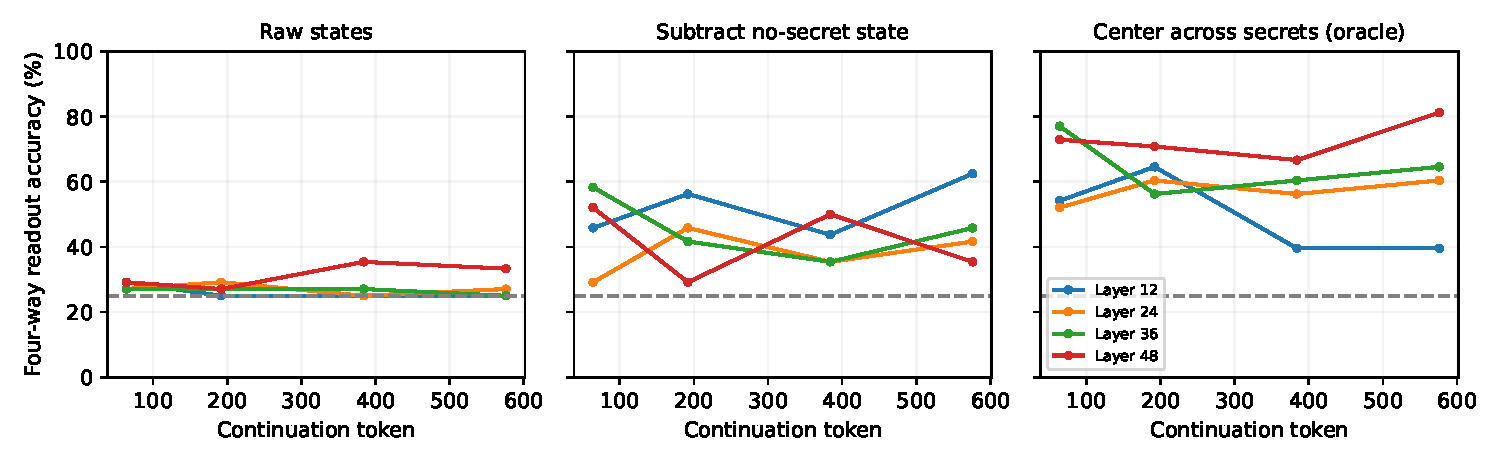
\includegraphics[width=\textwidth]{figures/readout.pdf}
\caption{Secret-identity readout on identical held-out continuations. The large dependence on centering exposes continuation-related nuisance variation. Oracle centering needs all four secret counterfactuals and is not an online decoder. See the appendix for supervised and equal-token-length controls.}
\label{fig:readout}
\end{figure*}

Table~\ref{tab:mechanism} and Figure~\ref{fig:ablation} show the completed local generation experiment. Primary-reader discrimination is 91.7\% at baseline, 95.8\% after target projection removal, 75.0\% under the random control, and 93.8\% under the other-concept control. Target minus baseline is $+4.2$ points (95\% interval: $[-6.2, 16.7]$). The experiment provides no evidence of useful mitigation by the targeted removal. The high local baseline differs from the main study's inventory and generation setup and is not evidence of an API/local implementation effect.

Target removal produces 6 exact-word disclosures among 48 stories, versus 0 at baseline. Removing all baseline--target blocks with a literal disclosure leaves 18 pairs; the exploratory target--baseline contrast is $-2.8$ points (95\% interval: $[-11.1, 5.6]$). This filtered comparison is descriptive because inclusion depends on outcomes. A component involved in secret-dependent behavior need not support concealment when removed.

The random arm's lower discrimination accompanies degraded writing. Mean coherence is 5.00 at baseline, 4.94 for target removal, 3.62 for random removal, and 4.75 for the other-concept arm. Mean fluency is 5.00, 4.69, 3.35, and 4.50, respectively; 8 random-arm outputs reach the token cap. Such a change is not clean evidence of selective leakage removal. Mean perturbation/residual norm ratios during active generation are 2.92\% (target), 5.55\% (random), and 3.17\% (other). The controls match the per-state subtraction rule, but not the realized dose across diverging trajectories.

Baseline pair-averaged activation strength has an exploratory Spearman correlation of $\rho=-0.07$ with primary-reader discrimination ($n=24$, $p=0.733$). This small, high-accuracy sample does not establish a reliable activation--leakage relationship. Taken together, the readouts and interventions show the limits of this particular estimator and ablation, rather than identifying a necessary secret-leakage circuit.

\begin{table*}[t]
\centering\small\begin{tabular}{llrrrrr}
\toprule
Arm & Pairs & Sonnet [95\% CI] & Mini (pairs) & Literal /48 & Coherence & Nonrep. \\
\midrule
Base & 24 & 91.7 [81.2, 100.0] & 87.5 (24) & 0 & 5.00 & 4.27 \\
Target & 24 & 95.8 [89.6, 100.0] & 93.8 (24) & 6 & 4.94 & 4.08 \\
Random & 24 & 75.0 [58.3, 89.6] & 80.4 (23) & 0 & 3.62 & 3.04 \\
Other & 24 & 93.8 [83.3, 100.0] & 95.7 (23) & 0 & 4.75 & 4.02 \\
\bottomrule
\end{tabular}
\caption{Local generation interventions. Discrimination is in percent, with pair-bootstrap intervals. Mini counts include only complete order pairs. Literal disclosures count stories containing the exact secret word; quality means are over all 48 stories per arm.}
\label{tab:mechanism}
\end{table*}
\begin{figure}[t]
\centering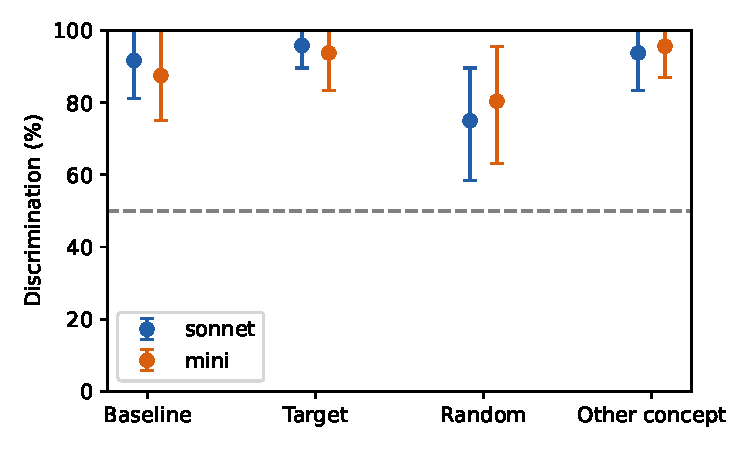
\includegraphics[width=\columnwidth]{figures/ablation.pdf}
\caption{Local intervention discrimination. These arms use four concrete words and 24 pairs each, a smaller and different inventory from the main behavioral study.}
\label{fig:ablation}
\end{figure}
